% arara: pdflatex
% arara: biber if (missing("bbl") || changed("bib"))
% arara: pdflatex if (missing("bbl") || changed("bbl"))
% arara: pdflatex if (found("log", "Label(s) may have changed."))
\documentclass[portuguese,10pt]{beamer}

\usepackage[version=3]{mhchem}

\usepackage[utf8]{inputenc}
\usepackage[T1]{fontenc}
\usepackage{polyglossia}
\setmainlanguage{portuges}
%\usepackage{microtype}
\usepackage{xcolor}
\usepackage{anyfontsize}
\usepackage{pdflscape}
\usepackage{bbding}

% -- Tipo de letra
%\usepackage[osf]{newpxtext}
%\usepackage{eulervm}
%\usepackage[scaled=1.05]{nimbusmononarrow}
\usepackage{fontspec}
\usepackage[sfdefault]{FiraSans} %% option 'sfdefault' activates Fira Sans as the default text font
\renewcommand*\oldstylenums[1]{{\firaoldstyle #1}}
\usepackage{FiraMono}
%\usepackage{newtxsf}

% -- Funções matemáticas extra
\usepackage{mathtools}
\usepackage{siunitx}

% -- Símbolos extra
\usepackage{amssymb}

\usepackage{textcomp}
\usepackage{gensymb}
\usepackage{cancel}

% -- Bibliografia
\usepackage[
	backend = biber,
	style = numeric,
	sorting = ynt
	]{biblatex}
\usepackage{fvextra}
\usepackage{csquotes}

% --  Definições de imagens
\usepackage{graphicx}
\graphicspath{{graphics/}}
\usepackage{svg}
\svgpath{{graphics/}}
\usepackage{caption}
\captionsetup{font=scriptsize}
\usepackage{subcaption}
\usepackage{afterpage}
\usepackage{tabularx}
%\usepackage[labelformat=empty]{caption}
\usepackage{multicol}
\usepackage{multirow}
\usepackage{booktabs}
\usepackage[export]{adjustbox}
\usepackage{caption}

% -- Desenhar circuitos elétricos e lógicos
\usepackage{tikz}
\usepackage{pgfplots}
\usetikzlibrary{arrows.meta,positioning,patterns}
\pgfplotsset{compat=1.5}
\pgfplotsset{table/search path = {data}}
\pgfplotsset{	/pgf/number format/use comma,}

\definecolor{ist-cyan}{cmyk}{1,0,0,0}
\definecolor{ist-gray}{cmyk}{0.2,0,0,0.8}

%\hypersetup{colorlinks,
%	linkcolor	= {white},
%	citecolor	= {ist-cyan},
%	urlcolor	= {ist-cyan}}

\usepackage{todonotes}

%%%%%%%%%%%%%%%%%%%%%%%%%%%%%%
%Cenas do beamer

%\addbibresource{main.bib}
\addbibresource{graphics.bib}
\definecolor{istblue}{cmyk}{1,0,0,0} % ist blue)

% símbolo de "certinho"
\def\checkmark{\tikz\fill[scale=0.4](0,.35) -- (.25,0) -- (1,.7) -- (.25,.15) -- cycle;} 
\mode<presentation>
{
  \usetheme{Madrid}       % or try default, Darmstadt, Warsaw, ...
  \usecolortheme{orchid} % or try albatross, beaver, crane, ...
  \usecolortheme[named=istblue]{structure}
  \usefonttheme{default}    % or try default, structurebold, ...
  \setbeamertemplate{navigation symbols}{}
  \setbeamertemplate{caption}[numbered]
  \setbeamertemplate{itemize items}[circle] %ball,circle, square
}

\setbeamertemplate{bibliography item}{\insertbiblabel}
\setbeamertemplate{caption}{\raggedright\insertcaption\par}

\setbeamertemplate{caption}[numbered]
\setbeamerfont{institute}{size=\Large}
\setbeamerfont{date}{size=\small}
\setbeamerfont{author}{size=\small}



\newrobustcmd*{\jamming}{\textit{jamming}}


\title[Guerra Eletrónica]{Guerra Eletrónica}

\author[MEAer -- Sistemas Aviónicos Integrados]{Pedro Afonso 66277 \and João Manito 73096 \and Daniel de Schiffart 81479}

\institute{Sistemas Aviónicos Integrados}
\date{Dezembro de 2018}
\setbeamertemplate{footline}
{
  \leavevmode%
  \hbox{%
  \begin{beamercolorbox}[wd=.333333\paperwidth,ht=2.25ex,dp=1ex,center]{author in head/foot}%
    \usebeamerfont{author in head/foot}\insertshortauthor
  \end{beamercolorbox}%
  \begin{beamercolorbox}[wd=.333333\paperwidth,ht=2.25ex,dp=1ex,center]{title in head/foot}%
    \usebeamerfont{title in head/foot}\insertshorttitle
  \end{beamercolorbox}%
  \begin{beamercolorbox}[wd=.333333\paperwidth,ht=2.25ex,dp=1ex,right]{date in head/foot}%
    \usebeamerfont{date in head/foot}\insertsection\hspace*{2em}
    \insertframenumber{} / \inserttotalframenumber\hspace*{2ex} 
  \end{beamercolorbox}}%
  \vskip0pt%
}

%%%%%%%%%%%%%%%%%%%%%%%%%%%%%%%%%%%%%%%%%%%%%%%%%%%%%%%%%%%%%%
\begin{document}

\begin{frame}
    \begin{figure}
	
\includegraphics[width=0.5\linewidth]{tecnico_logo.png}
    \end{figure}
    \titlepage
\end{frame}

\setbeamertemplate{section in toc}[circle]

\begin{frame}{Conteúdo}
  \tableofcontents
\end{frame}

\section{Introdução}

\begin{frame}{Introdução}
    In this research report we will present a general discussion on the topic of electric and electronic aeronautical systems and their presence within the context of war and warfare, beginning with an historical overview of the presence of these systems in aeronautics, their growth and expansion, the detection and exploitation of their vulnerabilities and subsequent and ongoing battle between exploitation and protection of these systems. Following it will be a presentation of the most notable weapons and systems within this topic, both historical and modern, which will culminate in a discussion on the future of electronic aeronautical systems and how relevant their overall protection can be to modern safety in the aeronautical and aerospace industry.
\end{frame}

\section{História}

\begin{frame}{História}
    \begin{itemize}
        \item Os primeiros incidentes ocorreram na guerra civil americana.
        \pause
        \item Soldados do exército confederado cortavam linhas de telégrafo das forças da união.
    \end{itemize}
    \begin{figure}[]
        \centering
        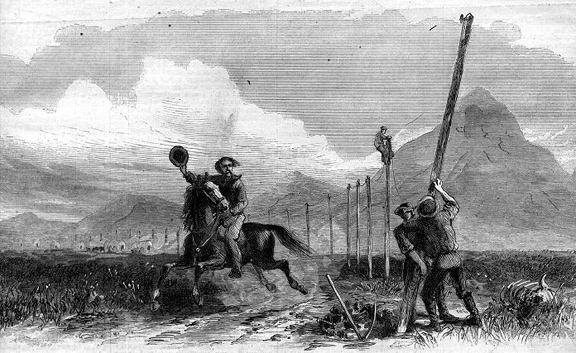
\includegraphics[width = 0.6\textwidth]{PoleA1}
        \caption{As primeiras linhas de telégrafo a serem construídas nos Estados Unidos \cite{polea1}.}
        \label{fig:polea1}
    \end{figure}
\end{frame}

\begin{frame}{Primeiro \textit{jamming} de rádio}
    \begin{minipage}[c]{0.6\linewidth}
        \begin{itemize}
            \item Com o aparecimento de sistemas de comunicação de rádio apareceu o \jamming{} intencional.
            \pause
            \item Numa corrida de iates da \textit{America's Cup}, um iate utilizou um transmissor mais potente para transmitir informação à imprensa para maior atenção e lucro.
            \item Foi a primeira instância de \jamming{} conhecida.
        \end{itemize}
    \end{minipage}
    \begin{minipage}[c]{0.39\linewidth}
        \begin{figure}[]
            \centering
            \includegraphics[width = \linewidth]{yachtrace}
            \caption{Corridas de iates americanos testemunharam o primeiro \jamming{} de rádio \cite{earlyradio}.}
            \label{fig:yachtrace}
        \end{figure}
    \end{minipage}
\end{frame}

\begin{frame}{Implementação militar}
    \begin{itemize}
        \item<1-> Os primeiros usos de \jamming{} de rádio militar foram treinadas pelo Reino Unido em 1902 e pelos Estados Unidos em 1903.
        \item<2-> As primeiras aplicações ocorreram na marinha.
        \item<3-> A guerra Russo-Japonesa entre 1904 e 1905 teve o primeiro grande uso de \jamming{} militar.
        \begin{itemize}
            \item Foi a primeira grande guerra onde ambas as partes utilizavam rádio para comunicações.
        \end{itemize}
    \end{itemize}
\end{frame}

\begin{frame}{Primeira Guerra Mundial}
    \begin{itemize}
        \item Comunicação por rádio na guerra manteve-se bastante primitiva.
        \item O pouco treino e hábito dos sistemas levou a pouco uso eficiente de \jamming{}.
        \item Ocorria bastante \jamming{} acidental entre forças aliadas devido a demasiadas transmissões num espaço reduzido.
    \end{itemize}
    \begin{figure}
        \centering
        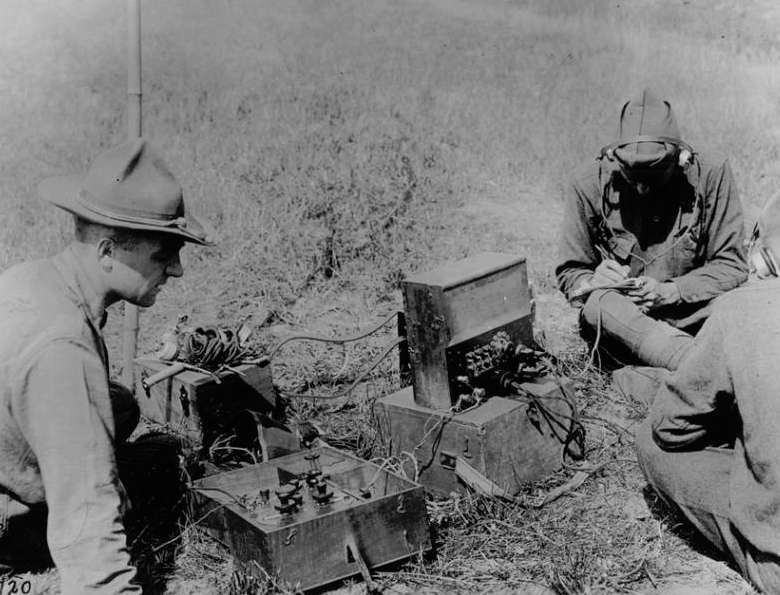
\includegraphics[width = 0.4\textwidth]{ww1}
        \caption{Primeiros aparelhos de rádio usados na Primeira Guerra Mundial \cite{worldwar1}.}
        \label{fig:ww1}
    \end{figure}
\end{frame}

\begin{frame}{Período Entre Guerras}
    No período após a Primeira Guerra Mundial, o potencial do rádio foi percebido e o desenvolvimento rápido.
    \begin{itemize}
        \item Transmissores diminuíram de tamanho e peso;
        \pause
        \item A sua performance melhorou;
        \pause
        \item A educação da população aumentou.
    \end{itemize}
    \pause
    Estes fenómenos levaram a uma melhoria dos sistemas de comunicação entre terra, mar e ar.
\end{frame}

\begin{frame}{Radar}
    Este período também viu o surgimento do radar.
    \begin{itemize}
        \item<1-> No início dos anos 1930, os radares conseguiam detetar alvos a 30 quilómetros.
        \item<2-> No fim da década, os radares aumentavam os seus alcances para mais de 160 quilómetros.
        \begin{itemize}
            \item O fator principal tornava-se a curvatura da Terra.
        \end{itemize}
        \item<3-> Também começavam a correr testes de \jamming{} de radar.
    \end{itemize}
    \begin{figure}
        \centering
        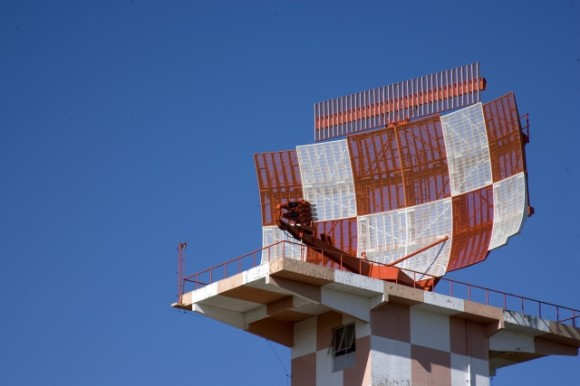
\includegraphics[width = 0.4\textwidth]{radarlisboa}
        \caption{Um transmissor-recetor de radar \cite{radarlisboa}.}
        \label{fig:radarlisboa}
    \end{figure}
\end{frame}

%\begin{frame}{Radar}
%    Por esta altura, o estudo de \jamming{} de radar foi cada vez mais desenvolvido.
%    \begin{itemize}
%        \item Os primeiros testes de tecnologias de \jamming{} começavam a ocorrer pela Europa, com os primeiros a serem feitos pela marinha inglesa em Londres.
%    \end{itemize}
%\end{frame}

\begin{frame}{Segunda Guerra Mundial}
    O rádio e os radares eram cada vez mais utilizados pelas forças armadas dos países europeus.
    \begin{itemize}
        \item A paragem de comunicação do inimigo teria cada vez mais importância no cenário da guerra.
        \item Rapidamente, a guerra tornou-se numa guerra de contra-medidas e contra-contra-medidas.
    \end{itemize}
\end{frame}

\begin{frame}{\textit{Battle Of The Beams}}
    Um cenário que ilustra esta natureza da guerra eletrónica é o período do \textit{Battle Of The Beams} entre a Alemanha e o Reino Unido.
    \begin{itemize}
        \item A Alemanha fez extensivo uso de radares para voar no escuro.
        \item Os radares utilizados serviam como um sistema de navegação primitivo.
        \item As forças aliadas foram apanhadas desprevenidas por bombardeamentos noturnos.
    \end{itemize}
\end{frame}

\begin{frame}{\textit{Knickebein}}
    A primeira fase deste período viu os alemães utilizarem uma variante do radar Lorenz.
    \begin{itemize}
        \item<1-> Este radar utiliza dois feixes para alinhar um avião com uma pista de aterragem.
        \item<2-> Os feixes apresentam características diferentes.
        \item<3-> Isto permite o piloto aterrar com segurança.
    \end{itemize}
    \begin{figure}
        \centering
        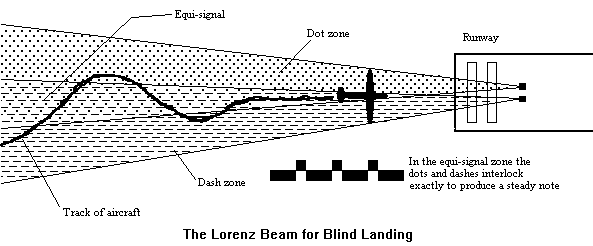
\includegraphics[width = 0.8\textwidth,trim = {0 8mm 0 0}, clip]{lorenz}
        \caption{Funcionamento do radar Lorenz \cite{pentagonknickebein}.}
        \label{fig:radarlisboa}
    \end{figure}
\end{frame}

\begin{frame}{\textit{Knickebein}}
    \begin{minipage}[c]{0.55\linewidth}
        \begin{itemize}
            \item<1-> Os dois radares foram utilizados pelos alemães para encontrar o alvo.
            \item<2-> Os britânicos redireccionaram os feixes de radar e emitiram réplicas próprias para desorientar os pilotos alemães.
            \item<3-> Isto causou despistes alemães e alguns pilotos até aterraram em solo inglês pensando que era a Alemanha.
        \end{itemize}
    \end{minipage}
    \hfill
    \begin{minipage}[c]{0.44\linewidth}
        \begin{figure}
            \centering
            {\tiny \includesvg[width = \textwidth]{Knickebein}}
            \caption{Mapa do uso do \textit{Knickebein} nos bombeamentos em Derby.}
        \end{figure}
    \end{minipage}
\end{frame}

\begin{frame}{Desenvolvimentos seguintes}
    \begin{itemize}
        \item As forças alemães desenvolveram novos sistemas de navegação via radar para combater a intervenção dos ingleses.
        \item Isto levou ao desenvolvimento dos radares \textit{X-Gerät} e mais tarde \textit{Y-Gerät}.
        \item A captura de aviões contendo esta tecnologia permitiu às forças inglesas bloquear as frequências utilizadas e impedir o uso destes radares.
        \item Este período terminou quando a força aérea alemã divergiu a sua atenção para a frente soviética.
        \item A \textit{Battle Of The Beams} ilustrou a natureza ataque-contra-ataque da guerra eletrónica.
    \end{itemize}
\end{frame}

\begin{frame}{Fim da Segunda Guerra Mundial}
    O fim da Segunda Guerra Mundial também viu o desenvolvimento e adopção de \textit{chaff}.
    \begin{figure}
        \centering
        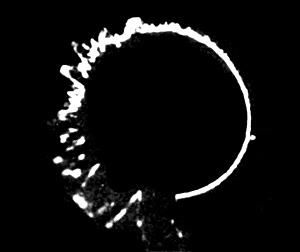
\includegraphics[width = 0.4\textwidth]{chaff}
        \caption{Exemplo de \textit{chaff} num \textit{display} de radar.}
    \end{figure}
    O uso de guerra eletrónica na frente do Pacífico também viu o uso de bastante \jamming{}, mas pouco desenvolvimento.
\end{frame}

\begin{frame}{Pós-Guerra}
    \begin{itemize}
        \item<1-> O período do pós-guerra viu muitas nações a considerarem a relevância do radar no campo de batalha.
        \item<2-> Começaram a ser definidos departamentos e oficiais dedicados à guerra eletrónica.
        \item<3-> Este período também viu o aparecimento primitivo do sector de \textbf{stealth}, o desenvolvimento de tecnologia para evitar deteção por radares anti-aéreos.
        \item<4-> O primeiro míssil auto-guiado \textit{surface-to-air} foi desenvolvido neste período inicial.
        \begin{itemize}
            \item Este levou ao desenvolvimento dos primeiros sistemas de \jamming{} de mísseis.
        \end{itemize}
    \end{itemize}
\end{frame}

\begin{frame}{Início da Guerra Fria}
    \begin{itemize}
        \item O início da guerra fria viu o confronto de inteligência entre os Estados Unidos da América e a União Soviética.
        \item Embora não houvesse confronto direto, ambas as partes faziam missões para obtenção de inteligência no inimigo.
        \item Com o risco de descoberta ser poder levar a resposta aprontada do inimigo, as missões eram realizadas com discreção extrema.
        \item Este período viu um investimento em tecnologia de obtenção de inteligência.
    \end{itemize}
\end{frame}

\begin{frame}{Missões ELINT}
    \begin{minipage}[c]{0.57\textwidth}
        \begin{itemize}
            \item As missões de obtenção de inteligência electrónica dos Estados Unidos começaram por esta altura.
            \item Utilizando aeronaves como o \textit{Lockheed U-2} obtiam informações sobre radares e sistemas de comunicação da União Soviética evitando deteção. Informações como
            \begin{itemize}
                \item Frequência de pulsação;
                \item Intervalo de tempo;
                \item Velocidade de \textit{scanning};
                \item Direcção de \textit{scanning};
                \item Localização de radares.
            \end{itemize}
        \end{itemize}
    \end{minipage}
    \hfill
    \begin{minipage}[c]{0.4\textwidth}
        \begin{figure}
            \centering
            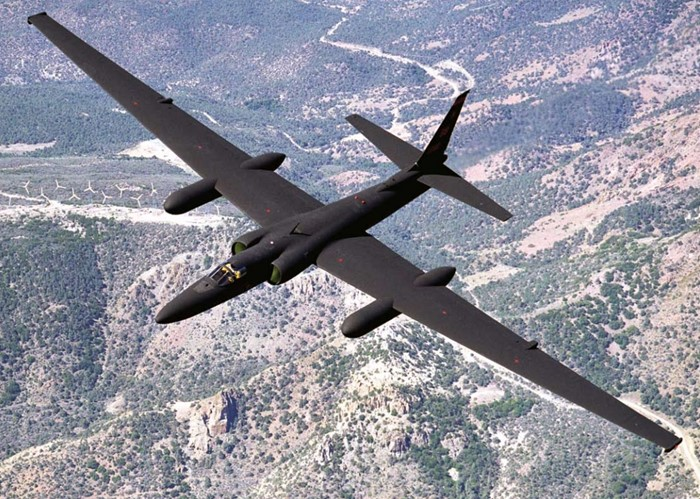
\includegraphics[width = \textwidth]{lockheedu2}
            \caption{O \textit{Lockheed U-2} utilizado pelos Estados Unidos.}
        \end{figure}
    \end{minipage}
    \vspace*{5mm}
    
    As missões terminaram quando um avião foi alvejado após detecção por tecnologia nova da União Soviética.
\end{frame}

\begin{frame}{A Guerra do Vietname}
    \begin{minipage}[c]{0.44\textwidth}
        \begin{figure}
            \centering
            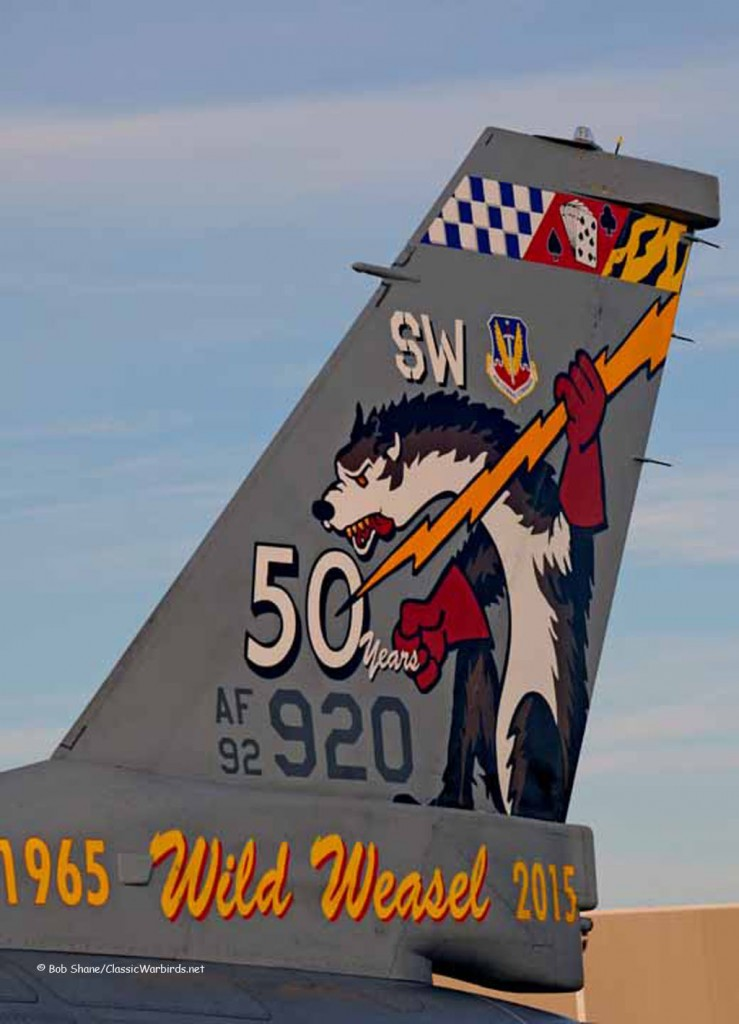
\includegraphics[width=\textwidth]{wildweasel}
            \caption{A cauda de um F-16 \textit{Wild Weasel}.}«
        \end{figure}
    \end{minipage}
    \hfill
    \begin{minipage}[c]{0.55\textwidth}
        \begin{itemize}
            \item Hello
        \end{itemize}
    \end{minipage}
\end{frame}

%----------------Pedro starts here ---------------------%


\section{Ataque Eletrónico}

\begin{frame}{Ataque Electrónico (AE) - Jamming }
    \begin{itemize}
        \item Mudando as características elétricas e magnéticas do ambiente;
        \vspace*{3mm}
        \item  Reduzindo a detectibilidade no radar e detectibilidade térmica da aeronave; 
        \vspace*{3mm}
        \item Nos dias actuais, o significado básico de ataque electrónico é o uso de vários sinais Jamming que afectam directamente os sistemas electrónicos na banda de radio frequência
    
    \end{itemize}
    
   
\end{frame}

\begin{frame}{Ataque Electrónico (AE) - Jamming }
    
    Jammer constítuido por: 
     \vspace*{5mm}
    \begin{itemize}
        \item Sistemas de controlo e suporte;
        \vspace*{3mm}
        \item  Um subsistema que produz sinais de Jamming; 
        \vspace*{3mm}
        \item Amplificadores de alta frequência e geradores com moduladores
         \vspace*{3mm}
         \item Dispositivos de Antena
    
    \end{itemize}
    
   
\end{frame}


\begin{frame}{Jammer automático}
    
\begin{figure}[ht]
\centering
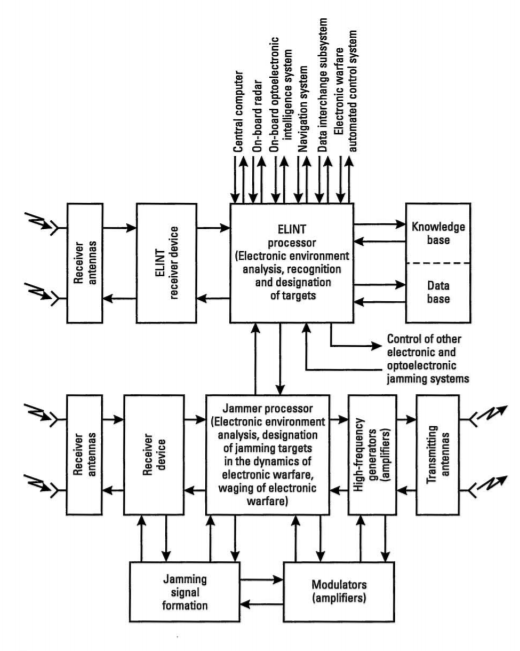
\includegraphics[width=0.4\textwidth]{jam1.png}
\caption{Diagrama de blocos para um Jammer automático}
\label{jam1}
\end{figure} 
\end{frame}



\begin{frame}{Jamming}
    
    Tipos de Jamming:
      \vspace*{5mm}
    \begin{itemize}
        \item Destrutivo;
        \vspace*{3mm}
        \item  Dissimulação; 
        \vspace*{3mm}
        \item Ilusão.
    
    \end{itemize}
    
   
\end{frame}



\begin{frame}{Jamming destrutivo }
    
      \vspace*{5mm}
    \begin{itemize}
    \item Potência da emissão de Jamming \begin{equation*}
P_{rec}= \frac{P_j G_j}{4 \pi D_j ^2} A_{rec} \gamma_j \eta_j    
\end{equation*}

\item Gama dinâmica limitada de receptores 
\begin{equation*}
K_{drr}= \frac{P_{rec max}}{P_{rec min}}    
\end{equation*}
$P_{rec min}$- limite de sensibilidade  $K_{drr}$ - gama dinâmica do receptor $D_j$ - distância do jammer ao alvo, $P_{rec max}$ - Potência radiada requerida para causar uma sobrecarga dinâmica
    \end{itemize}
    
  \end{frame}




\begin{frame}{Ataque Electrónico (AE) - Jamming}\Large
    
    
      \vspace*{5mm}
    \begin{itemize}
        \item Nível táctico - Destruição das defesas Anti-Aéreas num ataque
        \vspace*{6mm}
        \item  Nível Operacional - Simular dano nas defesas de forma a criar uma ilusão ao inimigo que realiza um ataque
        \vspace*{3mm}
     
    
    \end{itemize}
    \end{frame}

\begin{frame}{Jamming - Destrutivo}
    \begin{figure}[ht]
        \begin{minipage}[b]{0.49\linewidth}
            \centering
            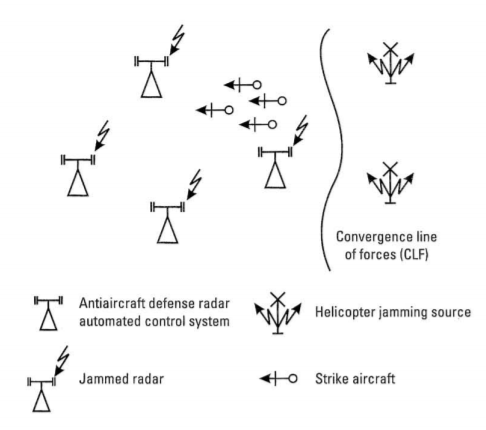
\includegraphics[width=40mm]{jam2.png}
            \caption{Métodos de ocultação aviões (helicópteros) e outros alvos de áreas fixas usando jamming}
            \label{jam2}
        \end{minipage}
        \hspace{\fill}
        \begin{minipage}[b]{0.49\linewidth}
            \centering
            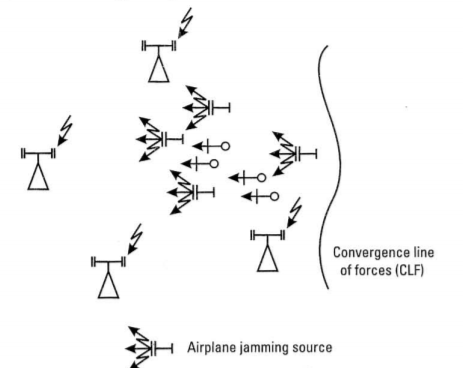
\includegraphics[width=40mm]{jam3.png}
            \caption{Métodos de observação de aviões em formação de batalha usando jamming.}
            \label{jam3}
        \end{minipage}
    \end{figure}
\end{frame}










%----------------Manito starts here ---------------------%
% para passar ha que pagar portagem que até se lixam...
\begin{frame}{Protecção Electrónica (PE)}
    \begin{itemize}
        \item Negar o efeito do jamming inimigo, mantendo capacidades operacionais aliadas;
        \vspace*{3mm}
        \item Ciclo contínuo de AE $\Rightarrow$ PE $\Rightarrow$ AE
        \vspace*{3mm}
        \item Vários métodos em uso, entre eles:
        \begin{itemize}
            \item Compressão de pulso
            \item Espectro de difusão em frequência variável
            \item Anulamento de lóbulo secundário
            \item Polarização
            \item Chaff
            \item Direccionamento por radiação
        \end{itemize}
    \end{itemize}
\end{frame}

\begin{frame}{Compressão de pulso}
    Exemplo: Radar de pulso
    \begin{itemize}
        \item<1-> Pulso sinusoidal de período T
        \item<1-> $SNR = \frac{K^2 A^2 T}{\sigma^2}$
        \item<1-> $\Delta R = \frac{1}{2} c \Delta T$
        \item<1-> Como reduzir efeitos de \textit{jamming}?
        \begin{itemize}
            \item<2-> Aumento do período do pulso
            \item<2-> Maior SNR
            \item<2-> Aumento da energia, diminuição da resolução de distância
        \end{itemize}
    \end{itemize}
\begin{figure}[ht]
\centering
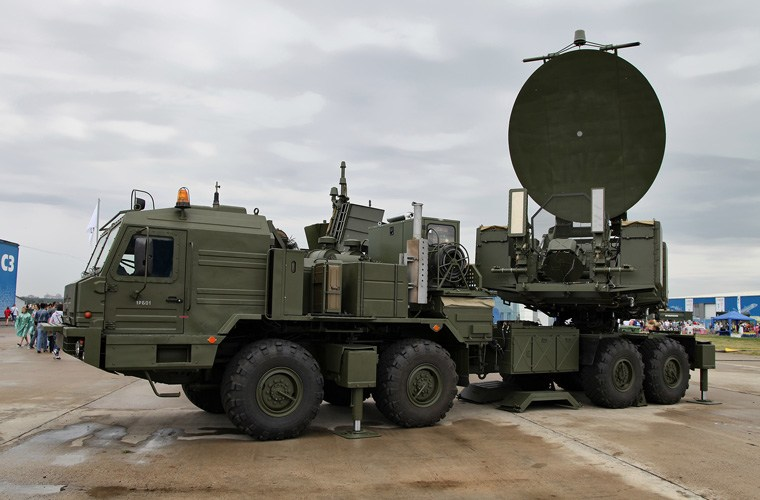
\includegraphics[width=0.4\textwidth]{graphics/jammer_militar.jpg}
\caption{\textit{Jammer} militar Krasukha-2}
\label{jammer_militar}
\end{figure}
\end{frame}

\begin{frame}{Compressão de pulso}
    Modulação linear em frequência do pulso - \textit{chirping}
    \begin{itemize}
        \item<1-> Modulação em torno da frequência da portadora, $f_0$
        \item<1-> Banda de modulação $\Delta f$
        \item<2-> Correlação centrada em $t=0$, aproximadamente função \textit{sinc}
        
    \end{itemize}
    \begin{figure}[ht]
\centering
\includegraphics[width=0.4\textwidth]{graphics/modulaçao_chirp.jpg}
\caption{Modulação do pulso em frequência - \textit{chirping}}
\label{modulacao_chirp}
\end{figure}
\end{frame}

\begin{frame}{Exemplo}
    \begin{figure}[ht]
        \begin{minipage}[b]{0.32\linewidth}
            \centering
            \includegraphics[width = \linewidth]{example-image}
            \caption{Label for a}
            \label{fig:3a}
        \end{minipage}
        \hspace{\fill}
        \begin{minipage}[b]{0.32\linewidth}
            \centering
            \includegraphics[width = \linewidth]{example-image}
            \caption{Label for b}
            \label{fig:3b}
        \end{minipage}
        \hspace{\fill}
        \begin{minipage}[b]{0.32\linewidth}
            \centering
            \includegraphics[width = \linewidth]{example-image}
            \caption{Label for c}
            \label{fig:3c}
        \end{minipage}
    \end{figure}
\end{frame}

\begin{frame}{Exemplo}
    \begin{figure}[ht]
        \begin{minipage}[b]{0.49\linewidth}
            \centering
            \includegraphics[width = \linewidth]{example-image}
            \caption{Label for a}
            \label{fig:2a}
        \end{minipage}
        \hspace{\fill}
        \begin{minipage}[b]{0.49\linewidth}
            \centering
            \includegraphics[width = \linewidth]{example-image}
            \caption{Label for b}
            \label{fig:2b}
        \end{minipage}
    \end{figure}
\end{frame}

\begin{frame}{Referências}
  \printbibliography
\end{frame}

\end{document}